\documentclass[10pt,a4paper,twocolumn,twoside]{article}
\usepackage[utf8]{inputenc}
\usepackage[catalan]{babel}
\usepackage{multicol}
\usepackage{graphicx}
\usepackage{fancyhdr}
\usepackage{times}
\usepackage{titlesec}
\usepackage{multirow}
\usepackage{lettrine}


\usepackage{xurl}
\PassOptionsToPackage{hyphens}{url}
\usepackage{hyperref}
\usepackage{breakurl}
\usepackage{subfig}

\usepackage[top=2cm, bottom=1.5cm, left=2cm, right=2cm]{geometry}
\usepackage[figurename=Fig.,tablename=Tabla]{caption}
\captionsetup[table]{textfont=sc}

\author{\LARGE\sffamily Marc Maldonado Lorca}
\title{\Huge{\sffamily Data Science: Estimación del peso de un cerdo}}
\date{}

\newcommand\blfootnote[1]{%
  \begingroup
  \renewcommand\thefootnote{}\footnote{#1}%
  \addtocounter{footnote}{-1}%
  \endgroup
}

%
%\large\bfseries\sffamily
\titleformat{\section}
{\large\sffamily\scshape\bfseries}
{\textbf{\thesection}}{1em}{}

\begin{document}

\fancyhead[LO]{\scriptsize Marc Maldonado Lorca: Estimación del peso de un cerdo}
\fancyhead[RO]{\thepage}
\fancyhead[LE]{\thepage}
\fancyhead[RE]{\scriptsize EE/UAB TFG INFORMÀTICA: Estimación del peso de un cerdo}

\fancyfoot[CO,CE]{}

\fancypagestyle{primerapagina}
{
   \fancyhf{}
   \fancyhead[L]{\scriptsize TFG EN ENGINYERIA INFORMÀTICA, ESCOLA D'ENGINYERIA (EE), UNIVERSITAT AUTÒNOMA DE BARCELONA (UAB)}
   \fancyfoot[C]{\scriptsize ``Febrer'' de 2022, Escola d'Enginyeria (UAB)}
}

%\lhead{\thepage}
%\chead{}
%\rhead{\tiny EE/UAB TFG INFORMÀTICA: Estimación del peso de un cerdo}
%\lhead{ EE/UAB \thepage}
%\lfoot{}
%\cfoot{\tiny{February 2015, Escola d'Enginyeria (UAB)}}
%\rfoot{}
\renewcommand{\headrulewidth}{0pt}
\renewcommand{\footrulewidth}{0pt}
\pagestyle{fancy}

%\thispagestyle{myheadings}
\twocolumn[\begin{@twocolumnfalse}

%\vspace*{-1cm}{\scriptsize TFG EN ENGINYERIA INFORMÀTICA, ESCOLA D'ENGINYERIA (EE), UNIVERSITAT AUTÒNOMA DE BARCELONA (UAB)}

\maketitle

\thispagestyle{primerapagina}
%\twocolumn[\begin{@twocolumnfalse}
%\maketitle
%\begin{abstract}
\begin{center}
\parbox{0.915\textwidth}
{\sffamily
\textbf{Resumen--}
Este proyecto se construye alrededor de la idea encontrar la mejor solución al problema de la estimación peso de un cerdo. Este desarrollo forma parte de un proyecto de Smart Farming impulsado por el Centro de Visión por Computador.
A partir del registro diario de una granja del peso de los cerdos y su correspondiente imagen de profundidad en el instante de la pesa se analizarán distintas soluciones basadas en aprendizaje computacional y se intentará maximizar la fiabilidad del sistema.
Analizaremos los pasos y las estrategias utilizadas hasta llegar a la mejor solución hasta el momento, fundamentada en el uso de CNNs y modelos regresivos.
\\
\\
\textbf{Palabras clave-- } Inteligencia Artificial, Aprendizaje Computacional, Aprendizaje Profundo, Visión por Computador, Granja Inteligente, Estimación Peso\\
\\
%\end{abstract}
%\bigskip
%\begin{abstract}
\bigskip
\\
\textbf{Abstract--} This project is built around the idea of finding the best solution to the problem of estimating the weight of a pig. This development is part of a Smart Farming project driven by the Computer Vision Center.
Based on a farm's daily record of pig weight and its corresponding depth image at the instant of weighing, different solutions based on computational learning will be analyzed and we will try to maximize the reliability of the system.
We will analyze the steps and strategies used to reach the best solution so far, based on the use of CNNs and regression models.
\\
\\
\textbf{Keywords-- } Artificial Intelligence, Machine Learning, Deep Learning, Computer Vision, Smart Farming, Weight Estimation\\
}

\bigskip

{\vrule depth 0pt height 0.5pt width 4cm\hspace{7.5pt}%
\raisebox{-3.5pt}{\fontfamily{pzd}\fontencoding{U}\fontseries{m}\fontshape{n}\fontsize{11}{12}\selectfont\char70}%
\hspace{7.5pt}\vrule depth 0pt height 0.5pt width 4cm\relax}

\end{center}

\bigskip
%\end{abstract}
\end{@twocolumnfalse}]

\blfootnote{$\bullet$ E-mail de contacte: maldonadolorcamarc@gmail.com}
\blfootnote{$\bullet$ Menció realitzada: Computació}
\blfootnote{$\bullet$ Treball tutoritzat per: Coen Antens (CVC)}
\blfootnote{$\bullet$ Curs 2021/22}

\section{Introducción - Contexto del trabajo}

\lettrine[lines=3]{D}{}esde hace unos años el sector agrario evoluciona junto a las nuevas tecnologías emergentes, lo que se conoce como Smart Farming. Este nuevo concepto deriva de la Industria 4.0, la cual aprovecha el potencial de las TIC para abaratar tanto los costes de producción como la eficiencia de las granjas. A partir de esta idea se han ideado nuevos modelos de gestión que van desde los invernaderos inteligentes y la gestión de plagas, hasta la implementación de drones agrícolas que utilizando imágenes aéreas permiten un ahorro significativo de tiempo y mano de obra a la hora de la verificación visual de un cultivo. Además no solo es aplicable al cultivo, sino que existe una interesante aplicación en el ganado.

Es por eso que el CVC trabajó en un proyecto de Smart Farming relacionado con la automatización de una granja de cerdos, donde uno de los retos pendientes era estimar el peso de los estos con la motivación de conocer su evolución y prepararlos para dar el peso óptimo en el matadero y así obtener la máxima rentabilidad posible. A la hora de entregar un cerdo al matadero su valor depende de lo que se aproxime su peso a loas 120 kg, este valor del animal disminuye tanto si su peso es inferior o superior al estándar establecido, es por eso que el control de la evolución de estos animales es tan importante para obtener beneficios.


Analizando el contexto, distribución de nuestra la granja y teniendo en cuenta el recorrido que realizaban los cerdos, se instaló en la báscula tradicional la cámara 3D Basler Blaze \cite{camara}, la cual se adapta bien por su resistencia, encargada de recoger el modelo 3D de los cerdos, con imágenes como la que se muestra en la \textbf{Fig \ref{foto}}, y su peso real, todo esto con la ayuda de células fotosensibles que controlarían la entrada individual de cada cerdo a la báscula, además de la instalación de un lector RFID y los respectivos PLC y PC, el montaje se muestra en las \textbf{Fig \ref{montaje}} para procesar y almacenar los datos obtenidos en formato Excel e imagen de profundidad. 

\begin{figure}[!htb]
\centering
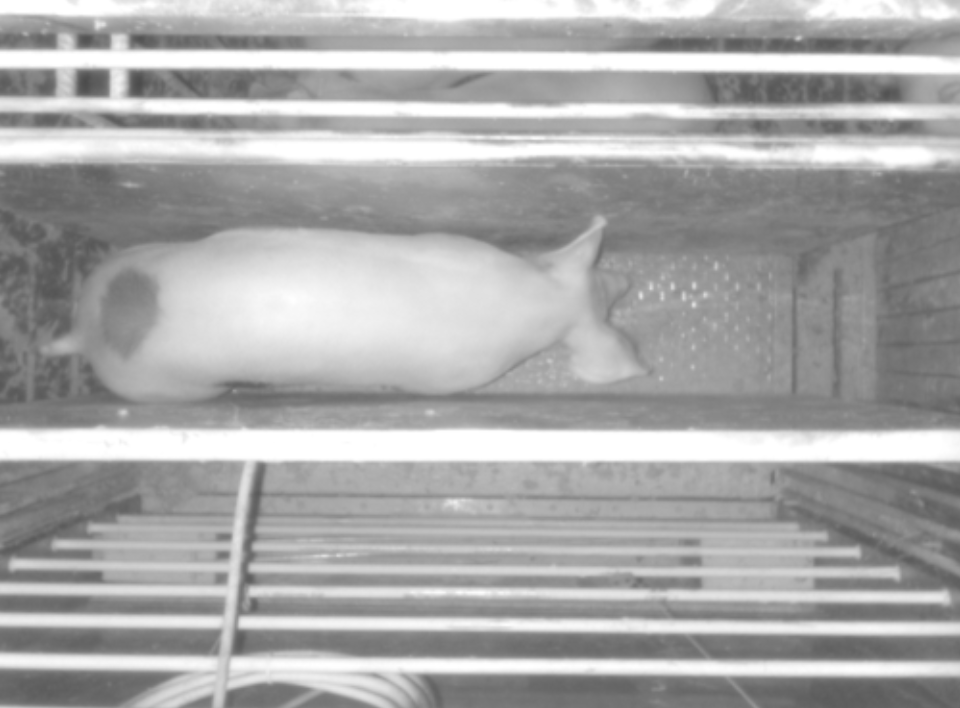
\includegraphics[width=0.4\textwidth]{05-TFG-template-latex/img/foto.png}
\caption{Ejemplo de imagen cenital}
\label{foto}
\end{figure}

\begin{figure}[!htb]
\centering
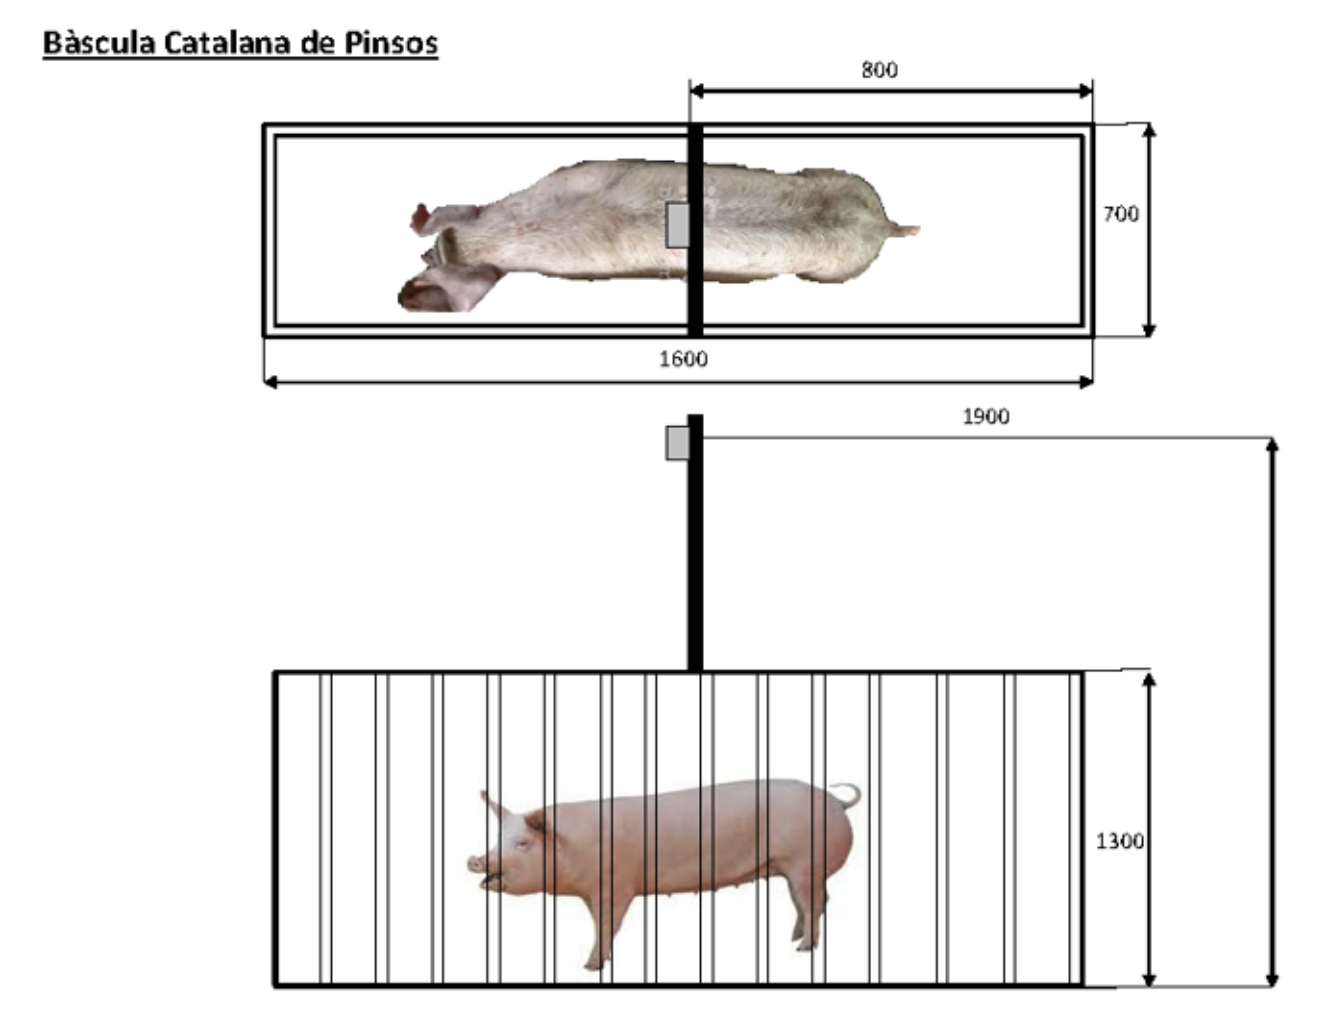
\includegraphics[width=0.4\textwidth]{05-TFG-template-latex/img/montaje.png}
\caption{Báscula con montaje de la cámara}
\label{montaje}
\end{figure}

Con todo este montaje y todos los datos generados damos puerta a este informe donde se desarrollará un modelo predictivo basado en aprendizaje profundo bajo el concepto de utilizar las imágenes y los datos para eliminar el costoso proceso de utilizar una báscula y agilizar el pesaje aumentando de esta manera el número de cerdos pesados por unidad de tiempo. \cite{sistema}.

\section{Estado del arte}
Este problema ya ha sido planteado por muchas personas, instituciones y empresas, además de haber sido abordado de distintas maneras y con distintos animales. Se han utilizado imágenes 2D donde se segmenta al cerdo utilizando técnicas de morfología, se construye su esqueleto y con las medidas de este utilizando una regresión se obtiene el peso \cite{Area}. En otro estudio usando vacas y una reconstrucción 3D similar a nuestros datos y extrayendo diferentes atributos como la altura, la anchura, el área, etc., consiguen estimar mediante regresión el peso de la vaca entre otros factores\cite{3D}.
También existe otra solución emplea imágenes de profundidad con las cuales utilizando redes neuronales convolucionales consigue estimar tanto el peso como otras variables biométricas del animal \cite{CNN}.
Finalmente otro estudio mediantes nubes de puntos como las que disponemos y analizando la postura de los cerdos, analizando la relación entre volumen y postura del animal consiguen mediante regresión estimar el peso.


Además de todos estos estudios ya existen productos en el mercado variados con diferentes enfoques.
La empresa Plf Agritech \cite{PLF} ha puesto en práctica diferentes tecnologías para el desarrollo de los animales en las granjas inteligentes, aportan una solución al problema de la detección de peso además de un alimentador automático inteligente y un control sobre el impacto medioambiental de estas grajas en términos de aire.
Fancom \cite{fancom} aparte de tener productos enfocados al crecimiento de otros animales como los pollos o productos destinados al cultivo de hongos también aportan una solución al control del peso de los cerdos con su producto Eyegrow \cite{fancomvideo}. Con una cámara de profundidad en el techo ellos son capaces de segmentar los cerdos individualmente y estimar el peso de ellos simultáneamente para después con la ayuda de un software poder analizar la evolución. Para esta tarea es interesarte leer un artículo de Sensors \cite{deteccion} que bajo el pretexto de la existencia de pocos datasets de cerdos ofrecen un modelo capaz de identificar a estos en fotos cenitales además de identificar la posición de sus distintas partes del cuerpo. Una aplicación similar a la anterior es la de Grostat \cite{GroStat}.


\begin{figure}[!htb]
\centering
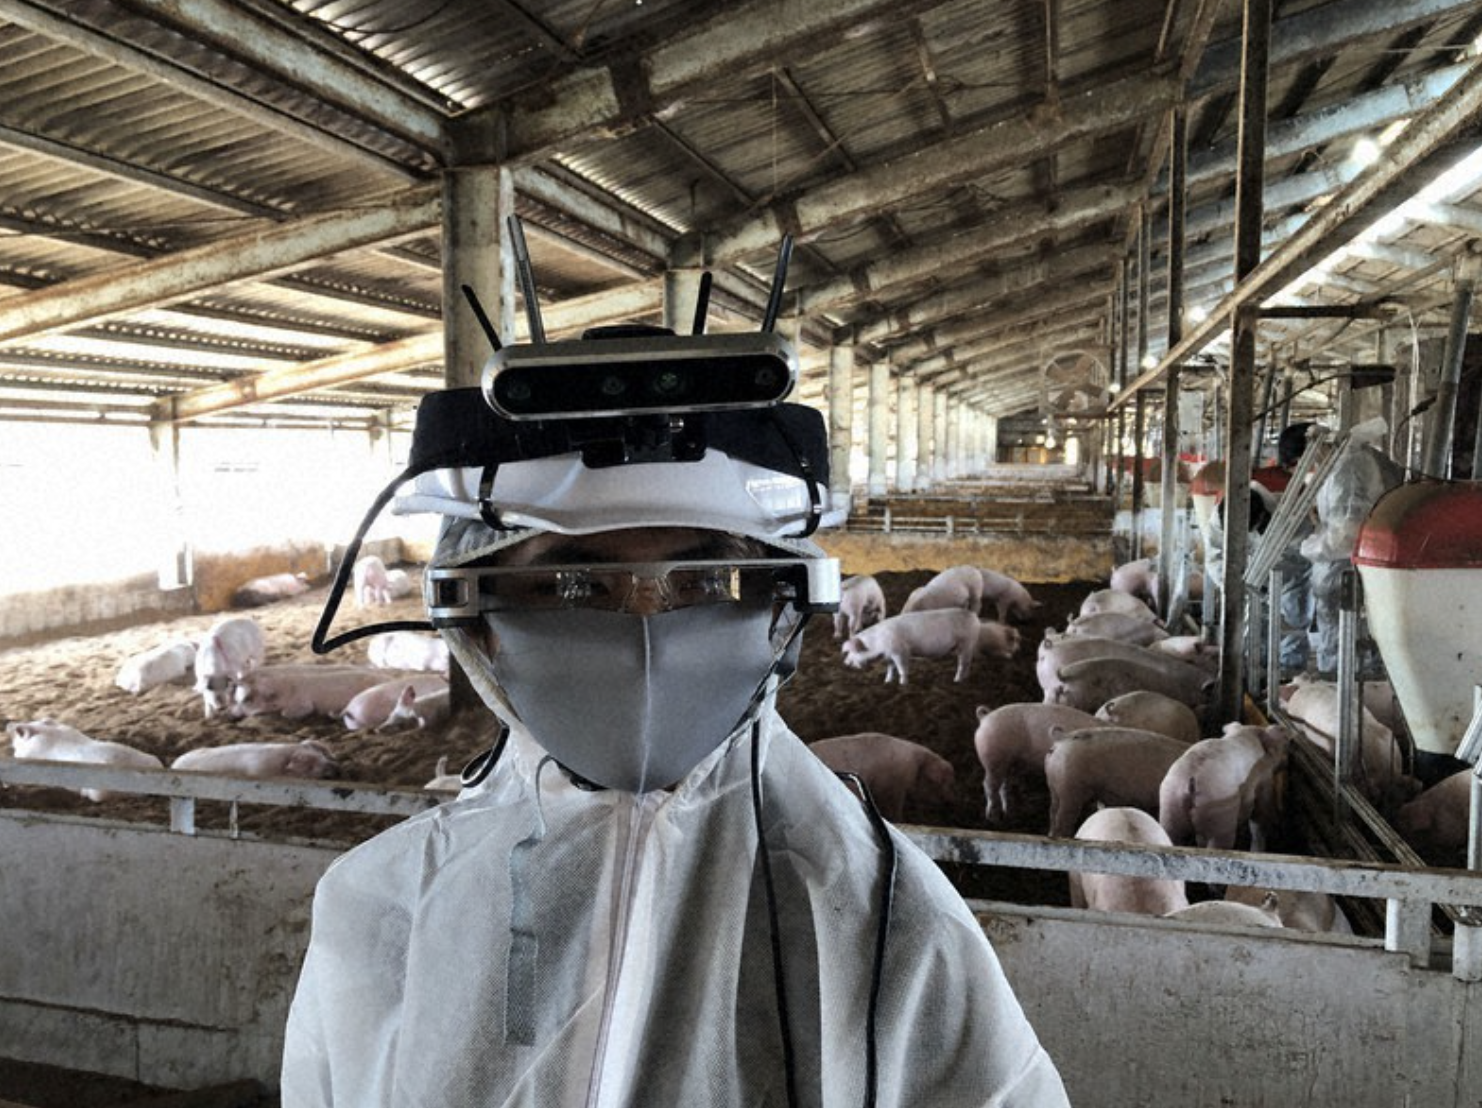
\includegraphics[width=0.5\textwidth]{05-TFG-template-latex/img/gafas.png}
\caption{Gafas de realidad virtual para la estimación de peso}
\label{gafas}
\end{figure}


Existe un enfoque diferente en cuanto a la manera de utilizar la cámara, mientras empresas como la anterior deciden colocar la cámara en un lugar fijo, otras empresas optan por la manipulación de la cámara de manera manual, de esta manera se facilitaría la selección del cerdo a pesar. Es el caso de H+L \cite{H+L} o Piggy Check \cite{piggycheck} que mediante cámaras 3D incorporadas en dispositivos móviles consiguen estimar los pesos de los cerdos de manera individual. Existe una solución similar desarrollada por Southwest Japan univ. \cite{japon}, pero esta vez la cámara está acoplada a unas GOOGLE glasses \cite{google} como se muestra en la \textbf{Fig \ref{gafas}} de manera que tan solo mirando al cerdo tendríamos la información, aunque todavía no se ha lanzado al mercado.
El peso es un buen indicador de la salud del cerdo, pero no es suficiente, Degree2Act \cite{degree} ha desarrollado un dispositivo para smartphone que mediante una cámara de temperatura nos informa de posibles enfermedades del cerdo, lo cual junto a una estimación del peso podría ser una potente herramienta.

Todas estas últimas soluciones propuestas por las empresas mencionadas utilizan redes neuronales, principalmente CNNs acompañadas con una gran variedad de imágenes en 3D registradas por la cámara, de esta manera consiguen soluciones robustas.

% Per a fer que la figura ocupi les dues columnes utilitzeu "figure*" per comptes de "figure"
% Utilitzeu el begin table només en cas de vole taules flotants. Si les voleu al lloc, tabular directament.


\section{Metodología}
Dentro de todas metodologías posibles para afrontar el proyecto se optó por una metodología ágil, concretamente Kanban, que al no tener que coordinar distintas personas es algo sencillo para el desarrollo de manera individual, estructurando las tareas en un panel cuatro columnas (Por hacer, Haciendo, Revisión y Hecho) donde se ordenan y clasifican según su estado.
Todo esto utilizando el software de Jira \cite{JIRA} que además de la gestión de tareas también proporciona herramientas como el diagrama de Gantt.
Para el proceso evolutivo del proyecto se siguió con las fechas planificadas para este además de reuniones semanales con el tutor en las cuales se comentaban avances semanales, definíamos siguientes puntos a los cuales atacar y se solucionaban dudas sobre el desarrollo

\section{Planificación}
La planificación del proyecto es algo que se ha ido adaptando y evolucionando al largo de este trabajo. Se dividió en distintas tareas que se han ido modificando, añadiendo nuevas y eliminando otras con tal de adaptarse a las necesidades del proyecto.
\subsection{Tareas}
Las tareas del proyecto divididas en sus distintos sprints son las siguientes:

\textbf{Sprint 1: }
\begin{itemize}
\itemsep0em 
\item \textbf{Tarea 1.1: }Estudio del dataset
\item \textbf{Tarea 1.2: }Visualización de los datos
\item \textbf{Tarea 1.3: }Segmentación clásica
\item \textbf{Tarea 1.4: }Conversión a nube de puntos
\item \textbf{Tarea 1.5: }Detección de objetos
\item \textbf{Tarea 1.6: }Segmentación semántica
\item \textbf{Tarea 1.7: }Limpieza de máscaras
\item \textbf{Tarea 1.8 : }Informe de progreso 1
    
\end{itemize}
\textbf{Sprint 2: }
\begin{itemize}
\itemsep0em 
    \item \textbf{Tarea 2.1: }Tratamiento datos de pesos
    \item \textbf{Tarea 2.2: }Estudio métodos de regresión
    \item \textbf{Tarea 2.3: }Entrenamiento CNNs regresión
    \item \textbf{Tarea 2.4: }Matching datos-imagen
    \item \textbf{Tarea 2.5: }Informe de progreso 2

    
\end{itemize}
\textbf{Sprint 3: }
\begin{itemize}
\itemsep0em 
    \item \textbf{Tarea 3.1: }Entrenamiento CNNs 2
    \item \textbf{Tarea 3.2: }Comparativa con otras soluciones
    \item \textbf{Tarea 3.3: }Análisis de resultados
    \item \textbf{Tarea 3.4: }Informe final
    \item \textbf{Tarea 3.5: }Presentación final

\end{itemize}

\subsection{Sprints}
Los sprints han sido marcados por las distintas entregas de los informes. De esta manera la carga de trabajo se ha repartido dependiendo del tiempo de duración del sprint y la disponibilidad de tiempo de trabajo para dedicar a cada tarea. Como se ha comentado anteriormente, además se han hecho reuniones semanales durante todos los sprints no solo para el análisis del progreso, sino también para realizar modificaciones de las tareas, compartir ideas de desarrollo con el tutor y tomar decisiones respecto a la evolución del proyecto.
El diagrama de Gantt con las tareas repartidas se puede encontrar en el Apéndice \ref{gant}.

\subsection{Revisión de la planificación}

Se ha cumplido con la planificación en gran parte.
En la mitad del primer sprint hubo que modificar los tiempos, ya que la primera vez se planificó sin realmente conocer el tiempo real a dedicar a cada tarea así pues se ajustaron más los tiempos a la realidad. Después de esta primera replanificación se fueron modificando las tareas durante los demás sprints de manera natural y ágil.
Sin embargo, al ser una metodología ágil siempre ha habido modificaciones en las tareas, pero nada que se alejase mucho del esquema inicial planteado.
Se propusieron en primera instancia tareas relacionadas con la regresión del peso utilizando GNNs, los cuales se descartaron más adelante debido al desarrollo prematuro en el que se encuentra esta tecnología.
También hay tareas no plasmadas en el esquema que se realizaron. Estas tareas aparecían en relación con algunas ya existentes y la mayoría de ellas se podían considerar como parte de las ya planificadas, las demás tareas eran detalles pequeños los cuales no eran oportunos para mostrarlos en el mapa de tareas.

\section{Desarrollo}    
En esta sección se detallarán los avances del proyecto y las diferentes técnicas y herramientas exploradas para encontrar la mejor solución al problema.

\subsection{Preparación de los datos}
Para empezar a plantear la regresión primero hemos de analizar los datos.
Los datos proporcionados fueron los tres siguientes:
\begin{enumerate}

\item Imágenes cenitales infrarrojas
\item Imágenes cenitales de profundidad en 16 bits
\item XLS con la información del peso, chip del cerdo, hora del pesaje...
\end{enumerate}

Como ya hemos comentado anteriormente, para obtener estos datos se utilizó una báscula con una cámara junto a un PC con su PLD y lector RFID. De esta manera los cerdos con chips pasaban por un circuito de manera diaria donde para comer era necesario pasar por la báscula de uno en uno. Cuando el peso se estabiliza se toma una foto y se registra el peso con su correspondiente número serial y la fecha.


La primera tarea fue proceder a mapear las imágenes con los pesos correspondientes en el archivo \textit{XLSX}. Cada imagen consta con una serie de dígitos en el nombre que indican un \textit{timestamp} de cuando se tomó la fotografía. Estos instantes de tiempo no encajan con el tiempo que marca la entrada de los pesos en el archivo Excel, existe una diferencia de 4 min de delay. Con esta información se genera un archivo \textit{CSV} con el mapeo.
Después de este proceso se descartaron imágenes de las cuales no existía ninguna entrada relacionada, además de las imágenes anteriores al 6/05/21 las cuales eran tomadas de forma distinta a las demás.

\begin{figure}[!htb]
\centering
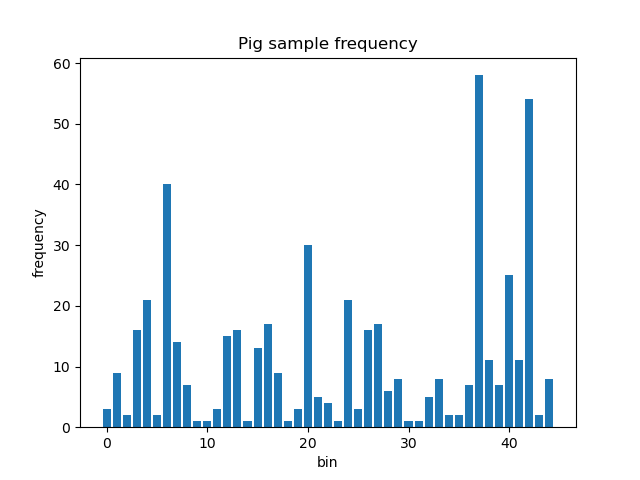
\includegraphics[width=0.5\textwidth]{05-TFG-template-latex/img/histogram.png}
\caption{Frecuencia de aparición de cada cerdo en los datos}
\label{hist}
\end{figure}

Una vez con esta información podemos consultar la frecuencia con la cual se pesa a cada cerdo independientemente para evaluar la fiabilidad de los datos, el histograma de la \textbf{Fig \ref{hist}} nos muestra la frecuencia de aparición de cada cerdo. Se puede observar que solo hay 3 cerdos de los cuales se hayan realizado más de 30 pesajes, lo cual nos puede comenzar a indicar que nuestros datos pueden estar sesgados en este aspecto. 
No obstante estas muestras se corresponden a un periodo de tiempo limitado, esto puede ser una explicación de los cerdos con pocas apariciones, que pueden haber sido pesados justo al inicio o al final de este periodo. No obstante las muestras deberían ser más homogéneas, indicando así u posible error en el circuito de pesado.

Seguidamente, se procedió a tratar los datos para así poder explotar su máximo potencial, eliminando información redundante y tratando de corregir todos los posibles errores.

\subsection{Segmentación}
La segmentación fue de las primeras ideas, con el objetivo de poder recortar cada cerdo de la imagen y así eliminar toda la información redundante para el cálculo del peso.

\subsubsection{Segmentación morfológica}

 Utilizar morfología para realizar una sustracción del fondo y así quedarnos con el cerdo recortado fue la primera opción, ya que todavía no se disponían de suficientes imágenes para poder recortar el cerdo mediante Machine Learning. En el primer momento de desarrollar una segmentación no se disponía de una imagen de la báscula vacía para ejecutar sustracciones de fondo, así que se intentó mediante la media de todas las imágenes generar una nueva la cual se usaría como fondo, esto se hizo tanto con las imágenes de la cámara de infrarrojos como con las imágenes de profundidad, estos métodos han sido bautizados como \textbf{Mean} y \textbf{Mean 3D} respectivamente. Una vez con esta nueva imagen generada se realiza una subtracción a cada imagen de cerdos para tratar de eliminar el fondo, antes habiéndole aplicado un suavizado gausiano para tratar de conseguir un resultado más limpio. Seguidamente probando thresholds manuales o utilizando Otsu\cite{Otsu}. Generamos la máscara final. Haciéndolo con las imágenes infrarrojas genera resultados notablemente mejores que con las imágenes de profundidad.
    
Seguidamente, se proporcionó una imagen de fondo para hacerle la subtracción, de la misma manera con las dos imágenes, estos métodos son los de \textbf{Difference} y \textbf{Difference3D}. Esta vez en vez de hacer la media de todas las imágenes realizamos la resta directamente con el fondo. De la misma manera se aplica un filtro de suavizado y con thresholds manuales y Otsu se generan las nuevas máscaras. Estas técnicas obtienen un rendimiento similar a las dos técnicas anteriores solo que a la inversa. En cuanto al uso de imágenes infrarrojas, este resultado se debe a que ahora a diferencia del anterior, utilizamos una imagen del fondo, debido a la superficie de la báscula se genera un reflejo de luz de un color similar al lomo del cerdo, así que la mayoría de los cerdos están segmentados por todo su cuerpo menos por la parte que coincide con el reflejo, esto explica la perdida de precisión. La mejora empleando imágenes de profundidad respecto al anterior método usando las mismas se debe a que existe una diferencia en el fondo de la imagen. Aquí es donde nos dimos cuenta de que una de las paredes de la báscula cambiada de posición dependiendo de la fotografía. Esto se debe a que las paredes se ajustan dependiendo del tamaño de los animales para no permitir que entren dos simultáneamente. Aun de esta manera de todas las imágenes disponibles existen un gran número con la pared en la misma posición respecto a demás imágenes con la pared en distinta posición. Al ser la imagen del fondo una representante las imágenes que más se repiten en cuanto a posición de la pared, por eso genera tan buenos resultados.

    Aquí es cuando probamos \textbf{Otsu} directamente con la imagen infrarroja, con las imágenes de profundidad queda directamente descartado, ya que segmentaría muchas partes de la báscula que para eliminarlas después utilizando morfología sería una tarea muy difícil. Hacerlo directamente con Otsu funciona bien pero no mejor que \textbf{Difference3D}.
    
    En este punto se puede ver que el verdadero problema se encuentra con el fondo y no con los cerdos así que se busca una solución, la primera es utilizar Canny y Hough\cite{hough} para detectar las líneas de la báscula y así eliminar el problema de las paredes móviles y el fondo. Esta técnica funcionó bien con el primer conjunto de imágenes, al tener nuevas se vuelve un reto imposible debido a la variedad de fotos, de este modo, se descarta y se opta por un recorte horizontal de la imagen que elimine fondo, pero no interfiera ni recorte en ningún caso alguna parte del cerdo, seguidamente aplica Otsu sobre el recorte. Hasta el momento esta técnica bautizada como \textbf{Otsu\_crop} se convierte en la mejor técnica para segmentar.
    
    También se experimenta usando Niblack y Sauvola \cite{Niblack}, pero no se obtienen ningún resultado a apreciar.
    
    \subsubsection{Segmentación por detección de objeto}
    
    \begin{figure}%
    \centering
    \subfloat[Groundtruth]{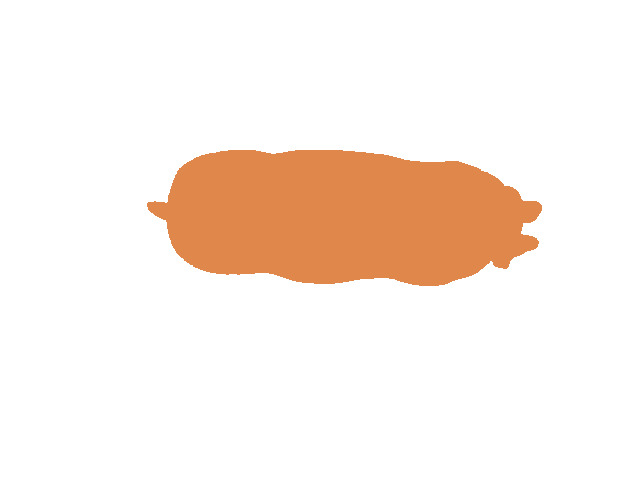
\includegraphics[scale=0.2]{05-TFG-template-latex/img/gt.jpg}\label{fig:a}}%
    \subfloat[Detección Objeto YOLO]{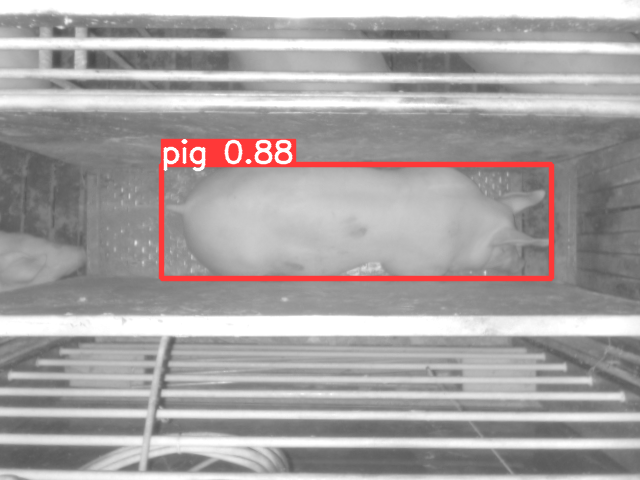
\includegraphics[scale=0.2]{05-TFG-template-latex/img/YOLOBOX.png}\label{fig:b}}\\
    \subfloat[Outsu aplicado al objeto YOLO]{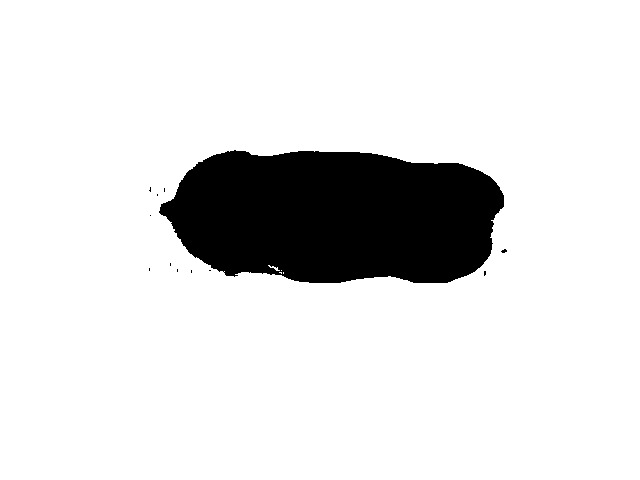
\includegraphics[scale=0.2]{05-TFG-template-latex/img/YOLO.jpg}\label{fig:c}}%
    \subfloat[Outsu refinado]{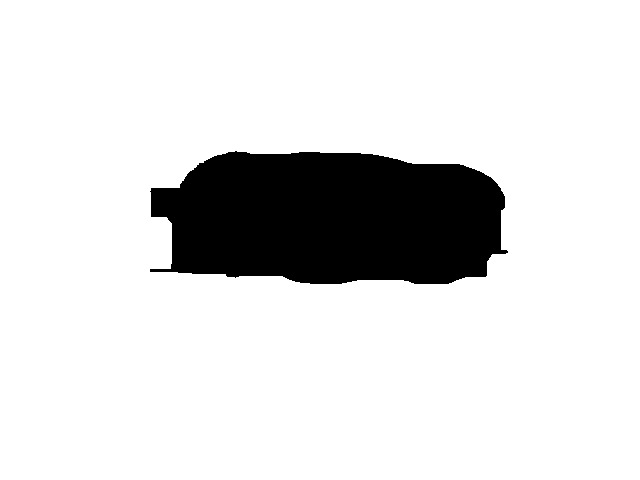
\includegraphics[scale=0.2]{05-TFG-template-latex/img/YOLOrefinado.jpg}\label{fig:d}}%
    \caption{Proceso de segmentación YOLO}%
    \label{yoloimg}%
    \end{figure}

    Viendo el potencial de recortar la imagen se decide generar \textit{groundtruths} para entrenar un modelo de segmentación semántica, para esto se utiliza la herramienta Hasty.ai \cite{hasty} la cual proporciona diversas herramientas para el etiquetado de imágenes, a nivel semántico, de objeto y de imagen. En este caso se hizo semánticamente, ya que a partir de aquí también podemos generar bounding boxes para la detección de objetos. Esta herramienta permite etiquetar de manera simultánea con demás personas y durante el etiquetado entrena modelos que te ofrecen una posible mascara la cual tú puedes editar. Con este groudtruth se extrajeron las bounding boxes y usando Google Colab se entrenó un modelo \textbf{Yolo}\cite{yolo}, concretamente V5, con el cual se recorta al cerdo y se aplica Otsu sobre la imagen recortada. Genera un resultado similar a Otsu\_crop, pero ligeramente peor en cuanto accuracy, de todas maneras elegimos Yolo porque la diferencia es ínfima y nos asegura que siempre cogemos al cerdo y no otros cerdos que asoman la cabeza por la puerta como se puede ver en alguna imagen. Además, sobre estas máscaras generadas se aplica técnicas de morfología para rellenar huecos dentro de los cerdos generados por las manchas de estos y kernels horizontales para tratar de dilatar horizontalmente la máscara y recuperar puntos pertenecientes al cerdo no segmentados. \cite{yolo} para con su detección tener una imagen recortada del cerdo y aplicar Otsu sobre él. El proceso de segmentación se puede ver en la \textbf{Fig \ref{yoloimg}} siendo \textbf{\subref{fig:a}} el \textit{groundtruth}, \textbf{\subref{fig:b}} la detección de Yolo, \textbf{\subref{fig:c}} Otsu aplicado sobre la detección de Yolo y \textbf{\subref{fig:d}} aplicando la morfología.
    
    \subsubsection{Segmentación semántica}
    
    Para encontrar una solución al problema de la segmentación se prepararon distintas arquitecturas . Se preparó para entrenar una U-Net\cite{unet} con el \textit{backbone} de ResNet-50\cite{resnet}, además de contemplar la opción de utilizar un modelo más ligero como MobileNetV2\cite{mobilenet}.
    Finalmente, tras distintas pruebas con diferentes \textit{backbones} y distintas configuraciones de los hiperparametros, se consiguió un modelo que entrenado con las imágenes captadas por la cámara infrarroja y las máscaras generadas con HastyAI\cite{hasty} obtenía unas métricas del 0.98 IOUScore\cite{iou} y 0.99 de accuracy usando como backbone InceptionV3\cite{inception}. Todo esto utilizando las imágenes recortadas manualmente para eliminar información que nunca será importante para la regresión y agilizar el entrenamiento del modelo.
\begin{table}[!b]
 \centering
\begin{tabular}{|c|c|}
\hline
\textbf{Método}          & \textbf{Acc} \\ \hline
Difference   & 0.47 \\ \hline
Difference3D & 0.87 \\ \hline
Mean         & 0.81 \\ \hline
Mean3D       & 0.36 \\ \hline
Otsu         & 0.69 \\ \hline
Otsu\_crop   & 0.97 \\ \hline
Yolo         & 0.97 \\ \hline
YOLO             & 0.97          \\ \hline
Segmentación semántica con cabeza  & 0.99          \\ \hline
Segmentación semántica  sin cabeza  & 0.99          \\ \hline
\end{tabular}
\caption{Resultados distintos métodos de regresión}
\label{resultadosSeg}
\end{table}

Más adelante en el desarrollo se decidió utilizar únicamente las imágenes de profundidad para entrenar el modelo de segmentación. No solo eso, sino que se generan las mismas máscaras, pero esta vez sin la cabeza de los cerdos para comprobar que la segmentación de esta parte del cuerpo del animal no sea una dificultad a la hora de estimar el peso. Se pueden consultar las métricas de la segmentación en la \textbf{Tabla \ref{resultadosSeg}}. Con estas métricas descartamos los métodos tradicionales planteados en el apartado utilizar este nuevo planteamiento
    
    \subsubsection{Otras transformaciones}
    
    Hemos descrito la manera en la que segmentamos los cerdos para así reducir la información y facilitar la tarea de regresión. Bajo la premisa de regularizar los datos se realiza una trasformación para centrar el cerdo en el centro de la imagen, es decir, se calcula el punto medio de la máscara recortada y se desplaza la imagen para centrarla.
    \begin{figure}
\centering
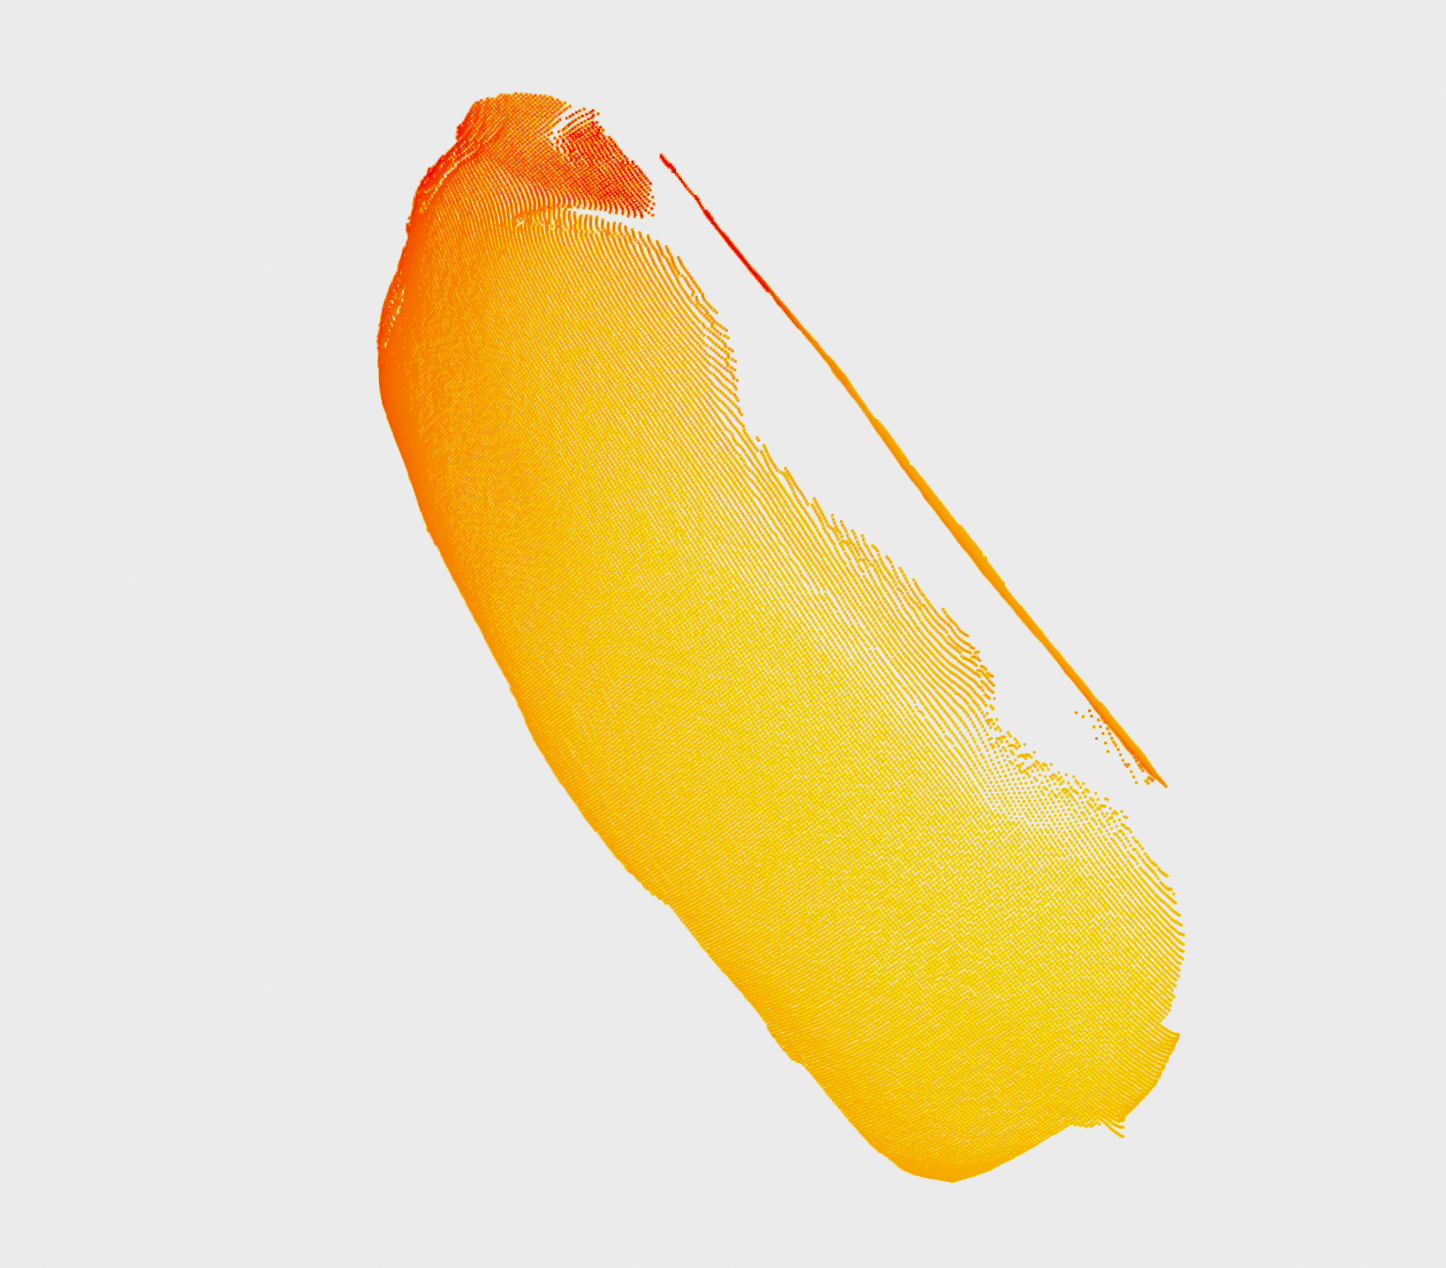
\includegraphics[width=0.3\textwidth]{05-TFG-template-latex/img/pcdmal.png}
\caption{Ejemplo de point cloud con pared}
\label{pcdmal}
\end{figure}

\begin{figure}
\centering
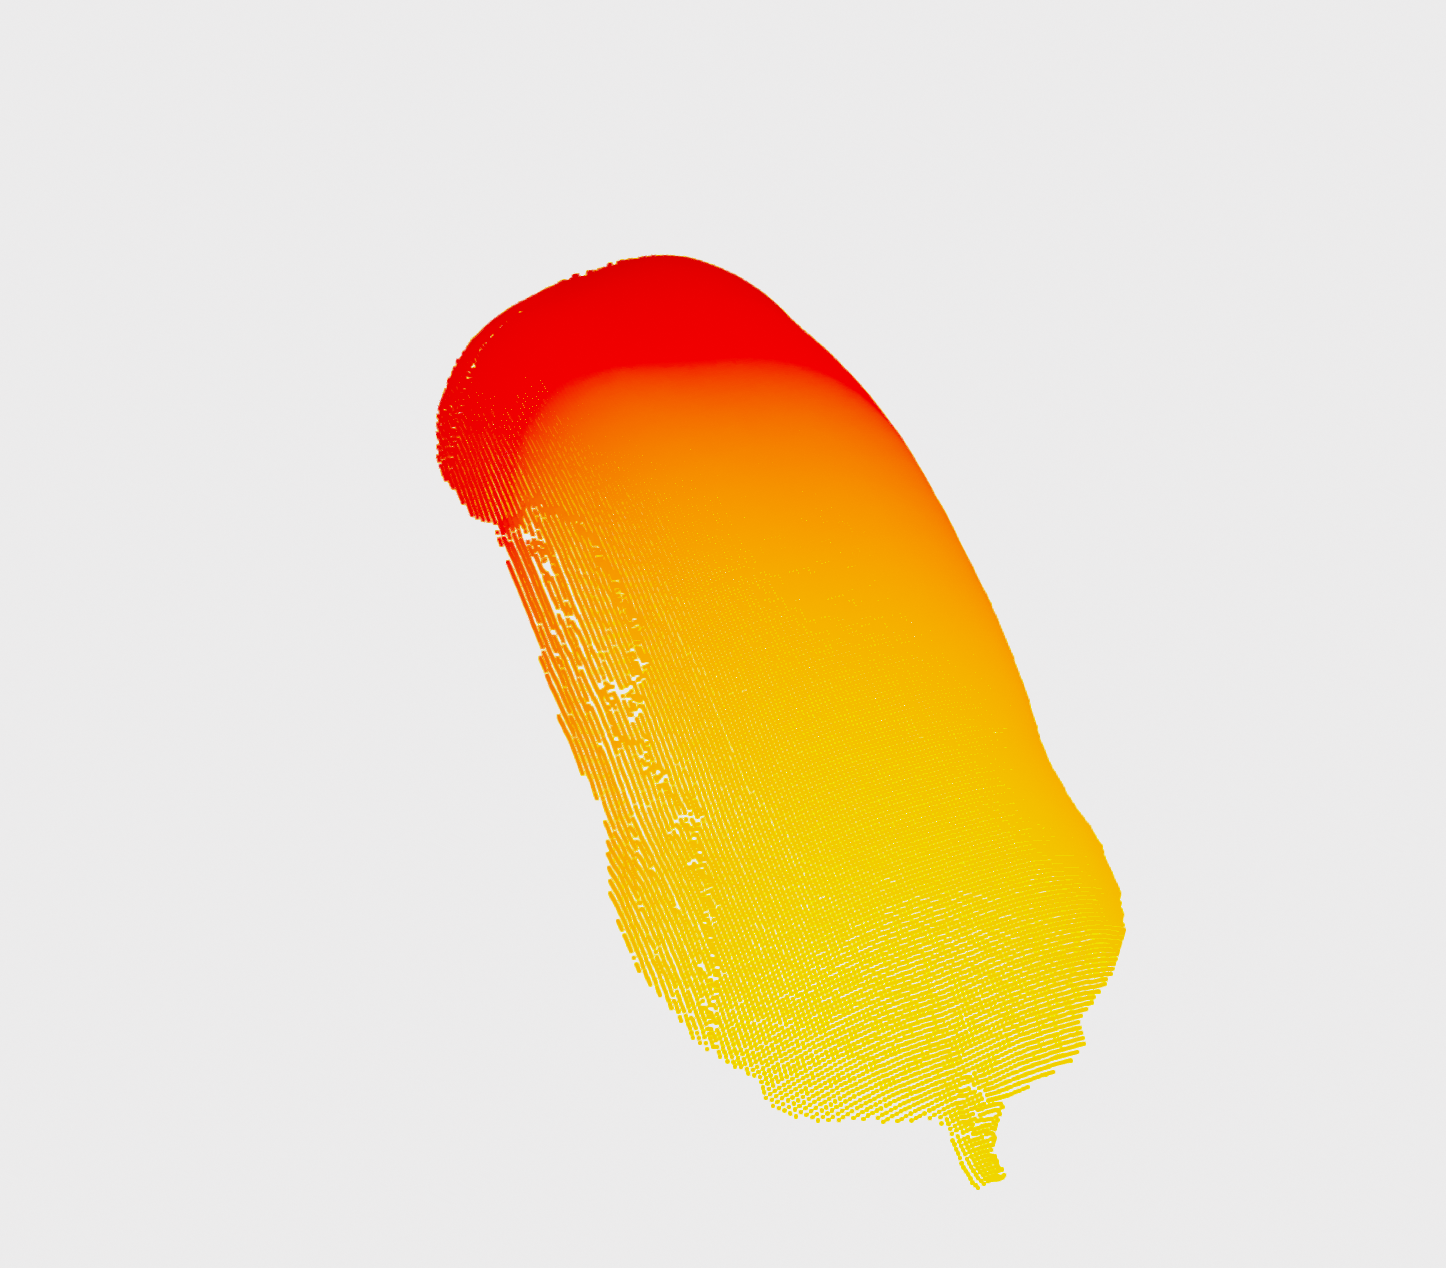
\includegraphics[width=0.3\textwidth]{05-TFG-template-latex/img/pcdbien.png}
\caption{Ejemplo de point cloud correcto}
\label{pcdbien}
\end{figure}
   Finalmente con la idea de utilizar GNNs para la estimación del peso, se construye el modelo en 3D del cerdo con Open3D \cite{open3D} y se eliminan todos los puntos que se encuentran más abajo de un determinado lindar para así eliminar suelo y outlayers de manera estadística par así eliminar los puntos segmentados no deseados. Sin embargo, esta técnica debe mejorarse, en algunos casos no se detecta correctamente toda la superficie del cerdo, en otros casos se seleccionan puntos pertenecientes a la pared de la báscula como en la \textbf{Fig \ref{pcdmal}}. Un ejemplo nube de puntos sin errores sería la que se muestra en la \textbf{Fig \ref{pcdbien}}.
   
Estas nubes de puntos fueron tratadas para transformarlas a un grafo en forma de mallas triangulares.
Para la tarea de construir las mallas se usó la librería Open3D\cite{open3D} que proporciona distintas funciones para la reconstrucción de superficies: \textit{Alpha shapes}, \textit{ball pivoting} y \textit{Poisson surface reconstruction}. Ajustando los parámetros de la función Poisson finalmente se consiguió la reconstrucción que se muestra en la \textbf{Fig \ref{mesh}}.

    \begin{figure}
    \centering
    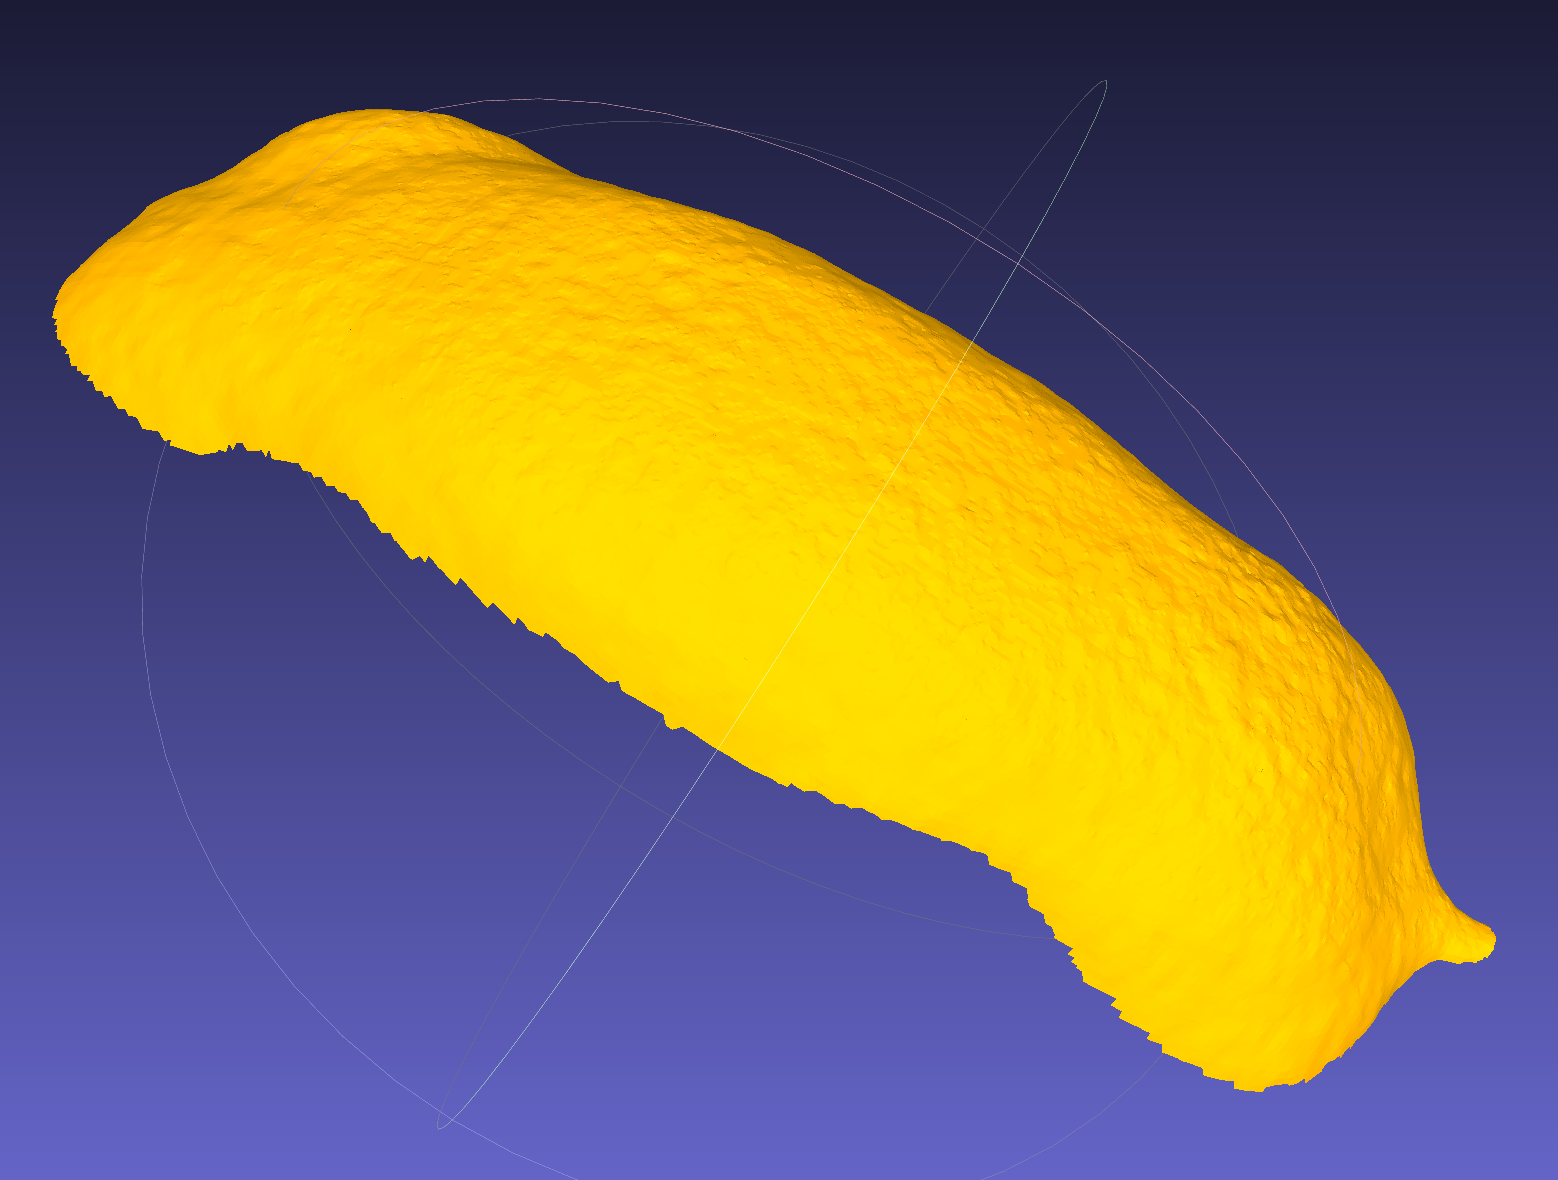
\includegraphics[width=0.4\textwidth]{05-TFG-template-latex/img/mesh.png}
    \caption{Malla generada con Poisson surface reconstruction}
    \label{mesh}
    \end{figure}
    
    Con estas nubes de puntos y estas mallas generadas se intentó buscar una solución al problema de regresión, pero se descartó debido a su complejidad y al escaso desarrollo existente de estas tecnologías en estos ámbitos. Se intentó adaptar el modelo de clasificación de PointNet\cite{pointnet} para regresión, no obstante no fue posible.
    
    
    
\subsection{Regresión}

En esta parte del desarrollo se procedió a entrenar un modelo capaz de estimar el peso del cerdo.

\subsubsection{Regresión Lineal}
Para la primera aproximación del peso se realizó una regresión linear con distintos atributos que parecieron interesantes a la hora de determinar el peso de un cerdo. Son los siguientes:

\begin{itemize}
\item \textbf{Área en pixeles: }Número de pixeles detectados como cerdo.
\item \textbf{Altura máxima: }Altura máxima de los pixeles detectados como cerdo.
\item \textbf{Área de la malla: }Área de la malla de triángulos generada.
\item \textbf{Altura media: }Altura media de los pixeles detectados como cerdo.
\item \textbf{Volumen aproximado: }Volumen aproximado del cerdo. Este se calcula ajustando los coeficientes de la fórmula elipsoide a los puntos de nuestro cerdo mediante buscando la configuración que minimice el error cuadrático. Una vez con la fórmula se procede al sampleo de distintos puntos de la elipse para generar un ConvexHull del cual podemos conocer su volumen. En la \textbf{Fig \ref{elipsoid}} se muestra un ejemplo de elipse ajustada al los puntos.
    
    \begin{figure}
    \centering
    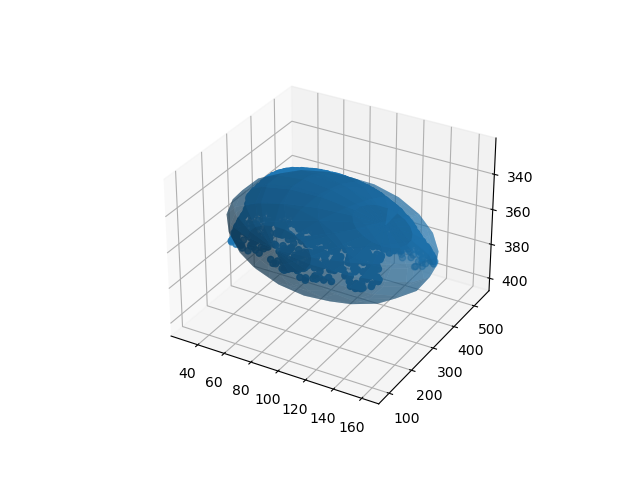
\includegraphics[width=0.5\textwidth]{05-TFG-template-latex/img/elipsoid.png}
    \caption{Elipsoide ajustada los puntos del cerdo}
    \label{elipsoid}
    \end{figure}
    
    Una vez entrenado este modelo con los datos normalizados observamos los coeficientes del modelo y nos revela la altura máxima es el atributo con el coeficiente más alto, es decir el más importante, seguido de la altura media y el número de pixeles.
    Esto nos aproxima a la siguiente solución utilizando las CNNs con un MAE\cite{mae} de 6.43kg.

\end{itemize}

\subsubsection{Regresión basada en CNN}
Se hicieron las primeras regresiones utilizando CNN con la ayuda de la librería ktrain\cite{ktrain}. Esta dispone de un \textit{early-stop} y ajustes automáticos del \textit{learning rate}, muy útiles para este proyecto, ya que al usar \textit{Google Colab} tenemos ejecuciones limitadas y de esta manera las conseguimos exprimir cada ejecución al máximo para sacar partido a la ventana de computación que nos presta este servicio.
\begin{figure*}[!]
 \centering
 \subfloat[Segmentación con cabeza]{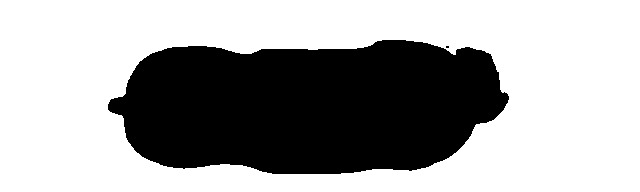
\includegraphics[scale=0.4]{05-TFG-template-latex/img/mask.jpg}\label{fig:a}}%
 \subfloat[Segmentación sin cabeza]{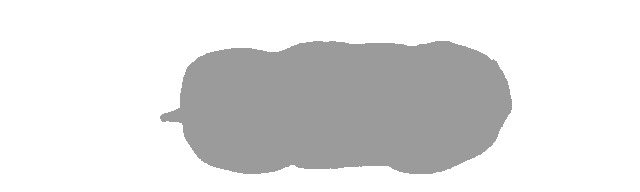
\includegraphics[scale=0.4]{05-TFG-template-latex/img/maskhead.jpg}\label{fig:b}}\
 \caption{Máscaras generadas por Segmentación semántica}%
 \label{masks}%
\end{figure*}
Primero se experimentó con las imágenes de profundidad en crudo y buscando mejorar estos resultados, surgió la idea de utilizar las máscaras de la segmentación sobre estas imágenes para eliminar la información irrelevante relacionada con el fondo.
Con los modelos entrenados, se revisaron las imágenes con un MAE\cite{mae} más elevado y se llegó a la conclusión de que posiblemente fueran las cabezas las que aportaban una gran varianza a estos resultados, de forma que los cerdos con la cabeza más escondida tendían a pesar menos y de manera contraria los cerdos con la cabeza más expuesta pesaban más. Para aplicar esta corrección se usan las máscaras de los cerdos sin cabeza. Las máscaras de los cerdos se pueden observar en la \textbf{Fig \ref{masks}} dónde (a) es la máscara teniendo en cuenta la cabeza y (b) sin esta.
Además, también se entrenó el modelo con los cerdos centrados en la imagen.
Se utilizaron también técnicas de data augmentation. Se probó añadiendo ruido gausiano a la imagen con la idea de hacer el modelo más robusto, pero solo empeoraba el resultado y se descartó. Lo que si funcionó correctamente y se utilizó durante el desarrollo es utilizar el vertical flip para aumentar datos, ya que un horizontal flip carecía de sentido, puesto que todos los cerdos estaba orientados de la misma manera.

Durante el desarrollo también surgió la idea de entrenar un modelo de clasificación capaz de clasificar cerdos según su tamaño, pequeños medianos y grandes, para así después crear modelos regresivos individuales para cada conjunto. Este modelo de clasificación obtiene un 84\% de accuracy, y con los modelos regresivos generados posteriormente a la clasificación podemos ver la mejora del MAE en los grupos de cerdos pequeños y grandes, en cambio, los medianos, al contener más clasificaciones erróneas, tanto de los pequeños como de los grandes, obtenemos un MAE bastante peor, que en promedio no mejora la estrategia de utilizar el conjunto de todas las imágenes para la regresión, así que por ese motivo se descartó este plan.


\begin{table}[!]
 \centering
\begin{tabular}{|c|c|}
\hline
\textbf{Método}          & \textbf{MAE (val)} \\ \hline
Imágenes raw             & 7.6          \\ \hline
Segmentación con cabeza  & 4.6          \\ \hline
Segmentación sin cabeza  & 4.5          \\ \hline
Centrado con cabeza & 4.2          \\ \hline
Centrado sin cabeza & 3.6          \\ \hline
\end{tabular}
\caption{Resultados de distintos métodos de regresión con 90\% de train}
\label{resultados}
\end{table}
En la \textbf{Tabla \ref{resultados}} se pueden consultar las métricas de los distintos métodos con el uso de CNN.

\section{Resultados}

Después de todas las pruebas realizadas y todas las mejoras podemos ver que el mejor método para estimar el peso del cerdo es utilizando las CNNs, concretamente manipulando los datos para que el cerdo se encuentre en el centro de la imagen y sin la cabeza segmentada, de esta manera conseguimos un MAE\cite{mae} de 3.6 en la validación utilizando el 90\% para el entrenamiento y el 10\% para la validación.
Reconociendo esto como la mejor configuración para resolver el problema nos planteamos conocer cuál sería la evolución de la loss a la hora de entrenar modificando las proporciones de datos usados para entrenar y validar. En la Tabla \textbf{Fig \ref{loss}} se muestra la variación del loss al modificar estas proporciones. Esta representación no es del todo correcta, ya que debido a limitaciones técnicas de falta de recursos no fue posible entrenar los modelos con cross validation para obtener resultados más fiables, de ahí las anomalías en el gráfico, de todas maneras se puede observar la tendencia a decrecer.

    \begin{figure}
    \centering
    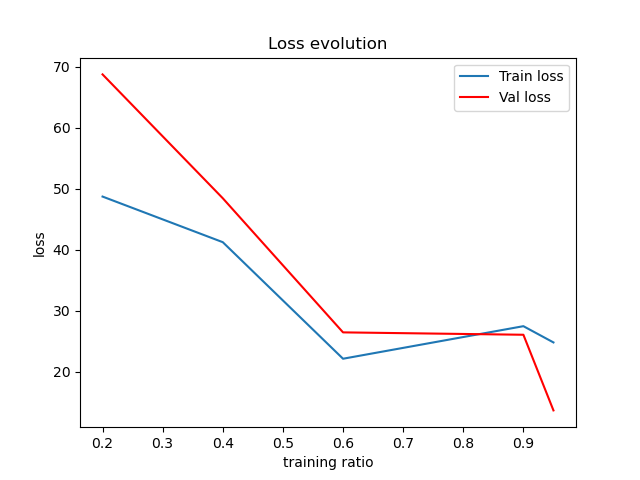
\includegraphics[width=0.55\textwidth]{05-TFG-template-latex/img/loss_evolution.png}
    \caption{Evolución del loss para distintas proporciones de train/val}
    \label{loss}
    \end{figure}

Por otro lado, en el Apéndice\ref{a3} se muestran las figuras correspondientes a los 3 cerdos con más muestras. Donde se describe el comportamiento de la mejor predicción utilizando CNNs y utilizando el método de regresión lineal, estas gráficas muestran la evolución del cerdo aplicando la técnica del moving average para eliminar el ruido y suavizar las gráficas.

    \begin{figure}
    \centering
    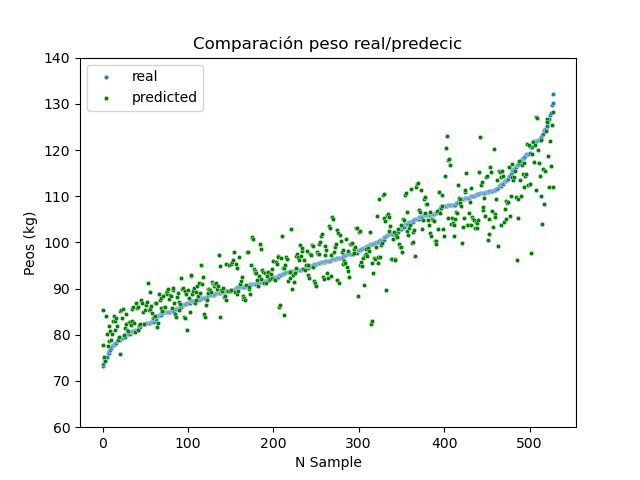
\includegraphics[width=0.55\textwidth]{05-TFG-template-latex/img/preds.png}
    \caption{Predicciones peso cerdos usando CNN}
    \label{grafico}
    \end{figure}
    
En la \textbf{Fig \ref{grafico}} correspondiente al método de segmentación con la máscara del cerdo completa podemos observar como las predicciones tienden a crear una línea horizontal en el plano, es decir, predecir un peso mayor para los cerdos pequeños y uno menor para los grandes, aunque con mucha desviación en los pesos grandes. También se pueden detectar puntos muy alejados de su peso real los cuales no podemos conocer si son ejemplos aislados de cerdos o errores en el registro de los datos.

En el siguiente enlace se puede encontrar el código fuente del proyecto:\\
\url{https://github.com/marcmaldonadolorca/Pig_weight_estimation.git}

\section{Conclusiones}

Finalmente, se concluye el proyecto habiendo desarrollado una herramienta capaz de estimar el peso de los cerdos.
Consideramos que es una solución válida para los datos proporcionados y con posible futura implementación en granjas inteligentes.
Tras distintos intentos y habiendo explotado todas las posibilidades que nos bridan los datos hemos sido capaces de generar un modelo capaz de predecir el peso con un MAE de 3.6kg con tan solo 600 muestras.
Respecto al tratamiento de los datos, se han explorado distintas soluciones a la hora de tratar las imágenes hasta encontrar la combinación que nos da mejores resultados. Acabamos eliminando el fondo el cual desde un primer momento pensábamos que podría introducir errores, hemos centrado el cerdo lo cual facilita la tarea para la CNN y finalmente no contamos con la cabeza en la segmentación del cerdo, ya que esta al variar tanto de posición acaba introduciendo un error que empeora nuestro resultado.

Por la parte de la regresión, todo indica a que con más muestras mejoraríamos el resultado sin importar el overfitting, por el hecho de que todas las fotos son tomadas en las mismas condiciones, es decir, la misma altura, el mismo ángulo, la misma luz, por lo cual no tendríamos problemas respecto a al sobreentrenamiento, puesto que estamos desarrollando el proyecto específicamente con las condiciones de esta granja. Sin embargo, el entrenamiento con más muestras para acercarnos más a nuestro objetivo no ha sido posible porque los datos pertenecen a la granja y dependemos de ellos para obtener más.
Además, se han detectado anomalías en los datos, irregularidades en el número de muestras de cada cerdo e imágenes sin entrada de peso. Esto nos abre la puerta a una búsqueda de errores en el sistema que registra los datos, al cual no tenemos acceso desde este proyecto. En el caso de existir errores con respecto a la obtención de datos sería otra justificación al error medio obtenido, de ser arreglado esta clase de problemas se podría mejorar la solución.

\subsection{Conclusiones generales}
De esta manera cerramos el proyecto satisfechos con el cumplimiento de los objetivos planteados al comenzarlo, pese no haber conseguido todo lo que esperábamos. Hemos cumplido con obtener el mejor error posible intentando sacarle partido a los datos, pero insatisfechos respecto a aplicar la tecnología de las GNN para la estimación del peso, lo cual se tuvo que descartar a mitad del proyecto debido a la nula información al respecto de la regresión numérica a partir de un grafo y el poco soporte de las GNNs existentes para su manipulación.
Respecto al tiempo empleado y a la planificación de tareas para el desarrollo consideramos que ha sido un punto fuerte a la hora de sacar el proyecto adelante. Debido a la flexibilidad que proporciona la metodología ágil y a la correcta estimación de las tareas hemos conseguido tener todo listo para la fecha final del proyecto.
La revisión del estado del arte ha sido un punto clave a la hora de orientar la solución. Como ya hemos comentado antes, debido a los recursos limitados no rivalizamos con las soluciones existentes comercializadas, pero sí que con más muestras obtendríamos una solución de calidad para la granja donde se está trabajando.

Este proyecto ha servido para poner en práctica todos los conocimientos asociados a este campo obtenido durante los estudios y a desarrollar técnicas de trabajo individuales y de búsqueda de información.

\subsection{Líneas futuras}
Para finalizar las conclusiones quiero mencionar las líneas futuras a las que se puede someter este proyecto. Como ya se ha citado anteriormente la primera ventana a la mejora es el uso de más datos proporcionados por la granja. Otra alternativa que queda pendiente es uno de los planteamientos iniciales con la utilización de GNN, para esta solución quizás se podrían instalar diversas cámaras para generar el modelo del cerdo en 3D y así ser más precisos. Finalmente otro punto sería hacer más robusta la solución, es decir, con más datos de entrenamiento y más variados podríamos obtener un producto como los mencionados en el estado del arte que sean capaces de estimar el peso de cualquier cerdo en cualquier condición, tanto de iluminación, como de posición de la cámara.
Otra opción es el uso de \textit{Long Short-term Memory}, redes capaces de obtener predicciones teniendo en cuenta los outputs pasados, de esta manera podremos obtener una predicción más acorde a la evolución del animal.

\section*{Agradecimientos}
Para acabar me gustaría agradecer este trabajo a todas esas personas que me han acompañado al largo de mis estudios, tanto profesores como alumnos.
También agradecer a mi familia por el apoyo y la motivación en estos tiempos de pandemia.
Finalmente agradecer al tutor de este proyecto Coen Antens por el tiempo dedicado y ayuda a lo largo de cada una de las etapas de este proyecto.


\begin{thebibliography}{11}


\bibitem{sistema}
    AHDB Pork \emph{"Pigs 2022 - Pig weighing systems"} [Online 30/9/2021] \\
    \url{https://www.youtube.com/watch?v=3CuLNYhFOjk}
    
\bibitem{camara}
    Basler \emph{"Basler blaze"} [Online 30/9/2021] \\
    \url{https://www.baslerweb.com/en/products/cameras/3d-cameras/basler-blaze/}

\bibitem{Area}
    K. Kollis, C.S. Phang, T.M. Banhazi and S.J. Searle \emph{"Weight estimation using image analysis and
    statistical modelling: A preliminary study"} [Online 30/9/2021] \\
    \url{https://www.researchgate.net/publication/236886740_Weight_Estimation_Using_Image_Analysis_and_Statistical_Modelling_A_Preliminary_Study}
\bibitem{3D}
    Dorota Anglart \emph{"Automatic estimation of body weight and body condition score in dairy cows using 3D imaging technique"} [Online 30/9/2021] \\
    \url{https://stud.epsilon.slu.se/6355/1/anglart_d_140114.pdf}
\bibitem{CNN}
    Jianlong Zhang, Yanrong Zhuang, Hengyi Ji, and Guanghui Teng \emph{"Pig Weight and Body Size Estimation Using a Multiple Output Regression Convolutional Neural Network: A Fast and Fully Automatic Method"} [Online 30/9/2021] \\
    \url{https://www.researchgate.net/publication/352102505_Pig_Weight_and_Body_Size_Estimation_Using_a_Multiple_Output_Regression_Convolutional_Neural_Network_A_Fast_and_Fully_Automatic_Method}
    
\bibitem{PLF}
    PLF Agritech \emph{"PLF Agritech"} [Online 30/9/2021] \\
    \url{http://plfag.com/technologies/}
    
\bibitem{fancom}
    Fancom \emph{"Fancom"} [Online 30/9/2021] \\
    \url{https://www.fancom.com}

\bibitem{fancomvideo}
    Fancom BV \emph{"eYeGrow - Weight monitor for finishers"} [Online 30/9/2021] \\
    \url{https://www.youtube.com/watch?v=CSuWWgY43PA}    

\bibitem{deteccion}
    Eric T. Psota, Mateusz Mittek, Lance Pérez and Ty B Schmidt \emph{"Multi-Pig Part Detection and Association with a Fully Convolutional Network"} [Online 30/9/2021] \\
    \url{https://www.researchgate.net/publication/352102505_Pig_Weight_and_Body_Size_Estimation_Using_a_Multiple_Output_Regression_Convolutional_Neural_Network_A_Fast_and_Fully_Automatic_Method}
    
\bibitem{GroStat}
    GroStat \emph{"GROWTH SENSOR"} [Online 30/9/2021] \\
    \url{http://grostat.com/growth_sensor.php#prettyPhoto}

\bibitem{H+L}
    H+L \emph{"optiSCAN"} [Online 30/9/2021] \\
    \url{https://hl-agrar.de/en_gb/optiscan/}

\bibitem{piggycheck}
    Agro Napló \emph{"Piggy Check – weigh pigs with your tablet PC"} [Online 30/9/2021] \\
    \url{https://www.agronaplo.hu/nagyvilag/piggy-check-weigh-pigs-with-your-tablet-pc}

\bibitem{japon}
    The Mainichi \emph{"Southwest Japan univ. develops smart glasses to visually estimate pigs' weight"} [Online 30/9/2021] \\
    \url{https://mainichi.jp/english/articles/20210601/p2a/00m/0na/007000c}

\bibitem{google}
    Glass \emph{"Glass"} [Online 30/9/2021] \\
    \url{https://www.google.com/glass/start/}

\bibitem{JIRA}
    Altassian \emph{"Jira"} [Online 30/9/2021] \\
    \url{https://www.atlassian.com/es/software/jira?}

\bibitem{degree}
    degree2act \emph{"degree2act"} [Online 30/9/2021] \\
    \url{https://www.degree2act.com/}
    

\bibitem{hasty}
    Hasty.ai \emph{"Hasty"} [Online 10/11/2021] \\
    \url{https://hasty.ai}



\bibitem{open3D}
    Open3D \emph{"Open3D"} [Online 10/11/2021] \\
    \url{http://www.open3d.org}

\bibitem{resnet}
    
    Kaiming He, Xiangyu Zhang, Shaoqing Ren and Jian Sun \emph{"Deep Residual Learning for Image Recognition"} [Online 10/11/2021] \\
    \url{https://arxiv.org/pdf/1512.03385.pdf}

\bibitem{mobilenet}
    Mark Sandler, Andrew Howard, Menglong Zhu, Andrey Zhmoginov and Liang-Chieh Chen \emph{"MobileNetV2: Inverted Residuals and Linear Bottlenecks"} [Online 10/11/2021] \\
    \url{https://arxiv.org/pdf/1801.04381.pdf}

\bibitem{unet}
    Olaf Ronneberger, Philipp Fischer and Thomas Brox \emph{"U-Net: Convolutional Networks for Biomedical Image Segmentation"} [Online 14/12/2021] \\
    \url{https://arxiv.org/pdf/1505.04597.pdf}
    
\bibitem{iou}
   pyimagesearch \emph{"Intersection over Union (IoU) for object detection"} \url{https://www.pyimagesearch.com/2016/11/07/intersection-over-union-iou-for-object-detection}
    [Online 14/12/2021] \\
    
\bibitem{inception}
    Christian Szegedy, Vincent Vanhoucke, Sergey Ioffe, Jonathon Shlens and Zbigniew Wojna \emph{"Rethinking the Inception Architecture for Computer Vision"} [Online 14/12/2021] \\
    \url{https://arxiv.org/pdf/1512.00567v3.pdf}
    
\bibitem{pointnet}
    Charles R. Qi, Hao Su, Kaichun Mo and Leonidas J. Guibas \emph{"PointNet: Deep Learning on Point Sets for 3D Classification and Segmentation"} [Online 14/12/2021] \\
    \url{https://arxiv.org/pdf/1612.00593.pdf}
    
\bibitem{ktrain}
    amaiya \emph{"amaiya/ktrain"} [Online 14/12/2021] \\
    \url{https://arxiv.org/pdf/1612.00593.pdf}


\bibitem{mae}
    Statistics How To \emph{"Absolute Error \& Mean Absolute Error (MAE)"} [Online 14/12/2021] \\
    \url{https://www.statisticshowto.com/absolute-error/}
    
\bibitem{Otsu}
    LearnOpenCV \emph{"Otsu’s Thresholding with OpenCV"} [Online 10/11/2021] \\
    \url{https://learnopencv.com/Otsu-thresholding-with-opencv/}

\bibitem{hough}
    LearnOpenCV \emph{"Hough Transform with OpenCV (C++/Python)"} [Online 10/11/2021] \\
    \url{https://learnopencv.com/hough-transform-with-opencv-c-python/}

\bibitem{hasty}
    Hasty.ai \emph{"Hasty"} [Online 10/11/2021] \\
    \url{https://hasty.ai}

\bibitem{yolo}
    Yolov5 \emph{"ultralytics/yolov5"} [Online 10/11/2021] \\
    \url{https://github.com/ultralytics/yolov5}

\bibitem{Niblack}
    scikit-image \emph{"Niblack and Sauvola Thresholding"} [Online 10/11/2021] \\
    \url{http://www.open3d.org}



\end{thebibliography}

\onecolumn
\appendix

\section*{Apéncide}

\setcounter{section}{1}

\subsection{Diagrama de Gantt}
\label{gant}

\begin{figure}[!htb]
\centering
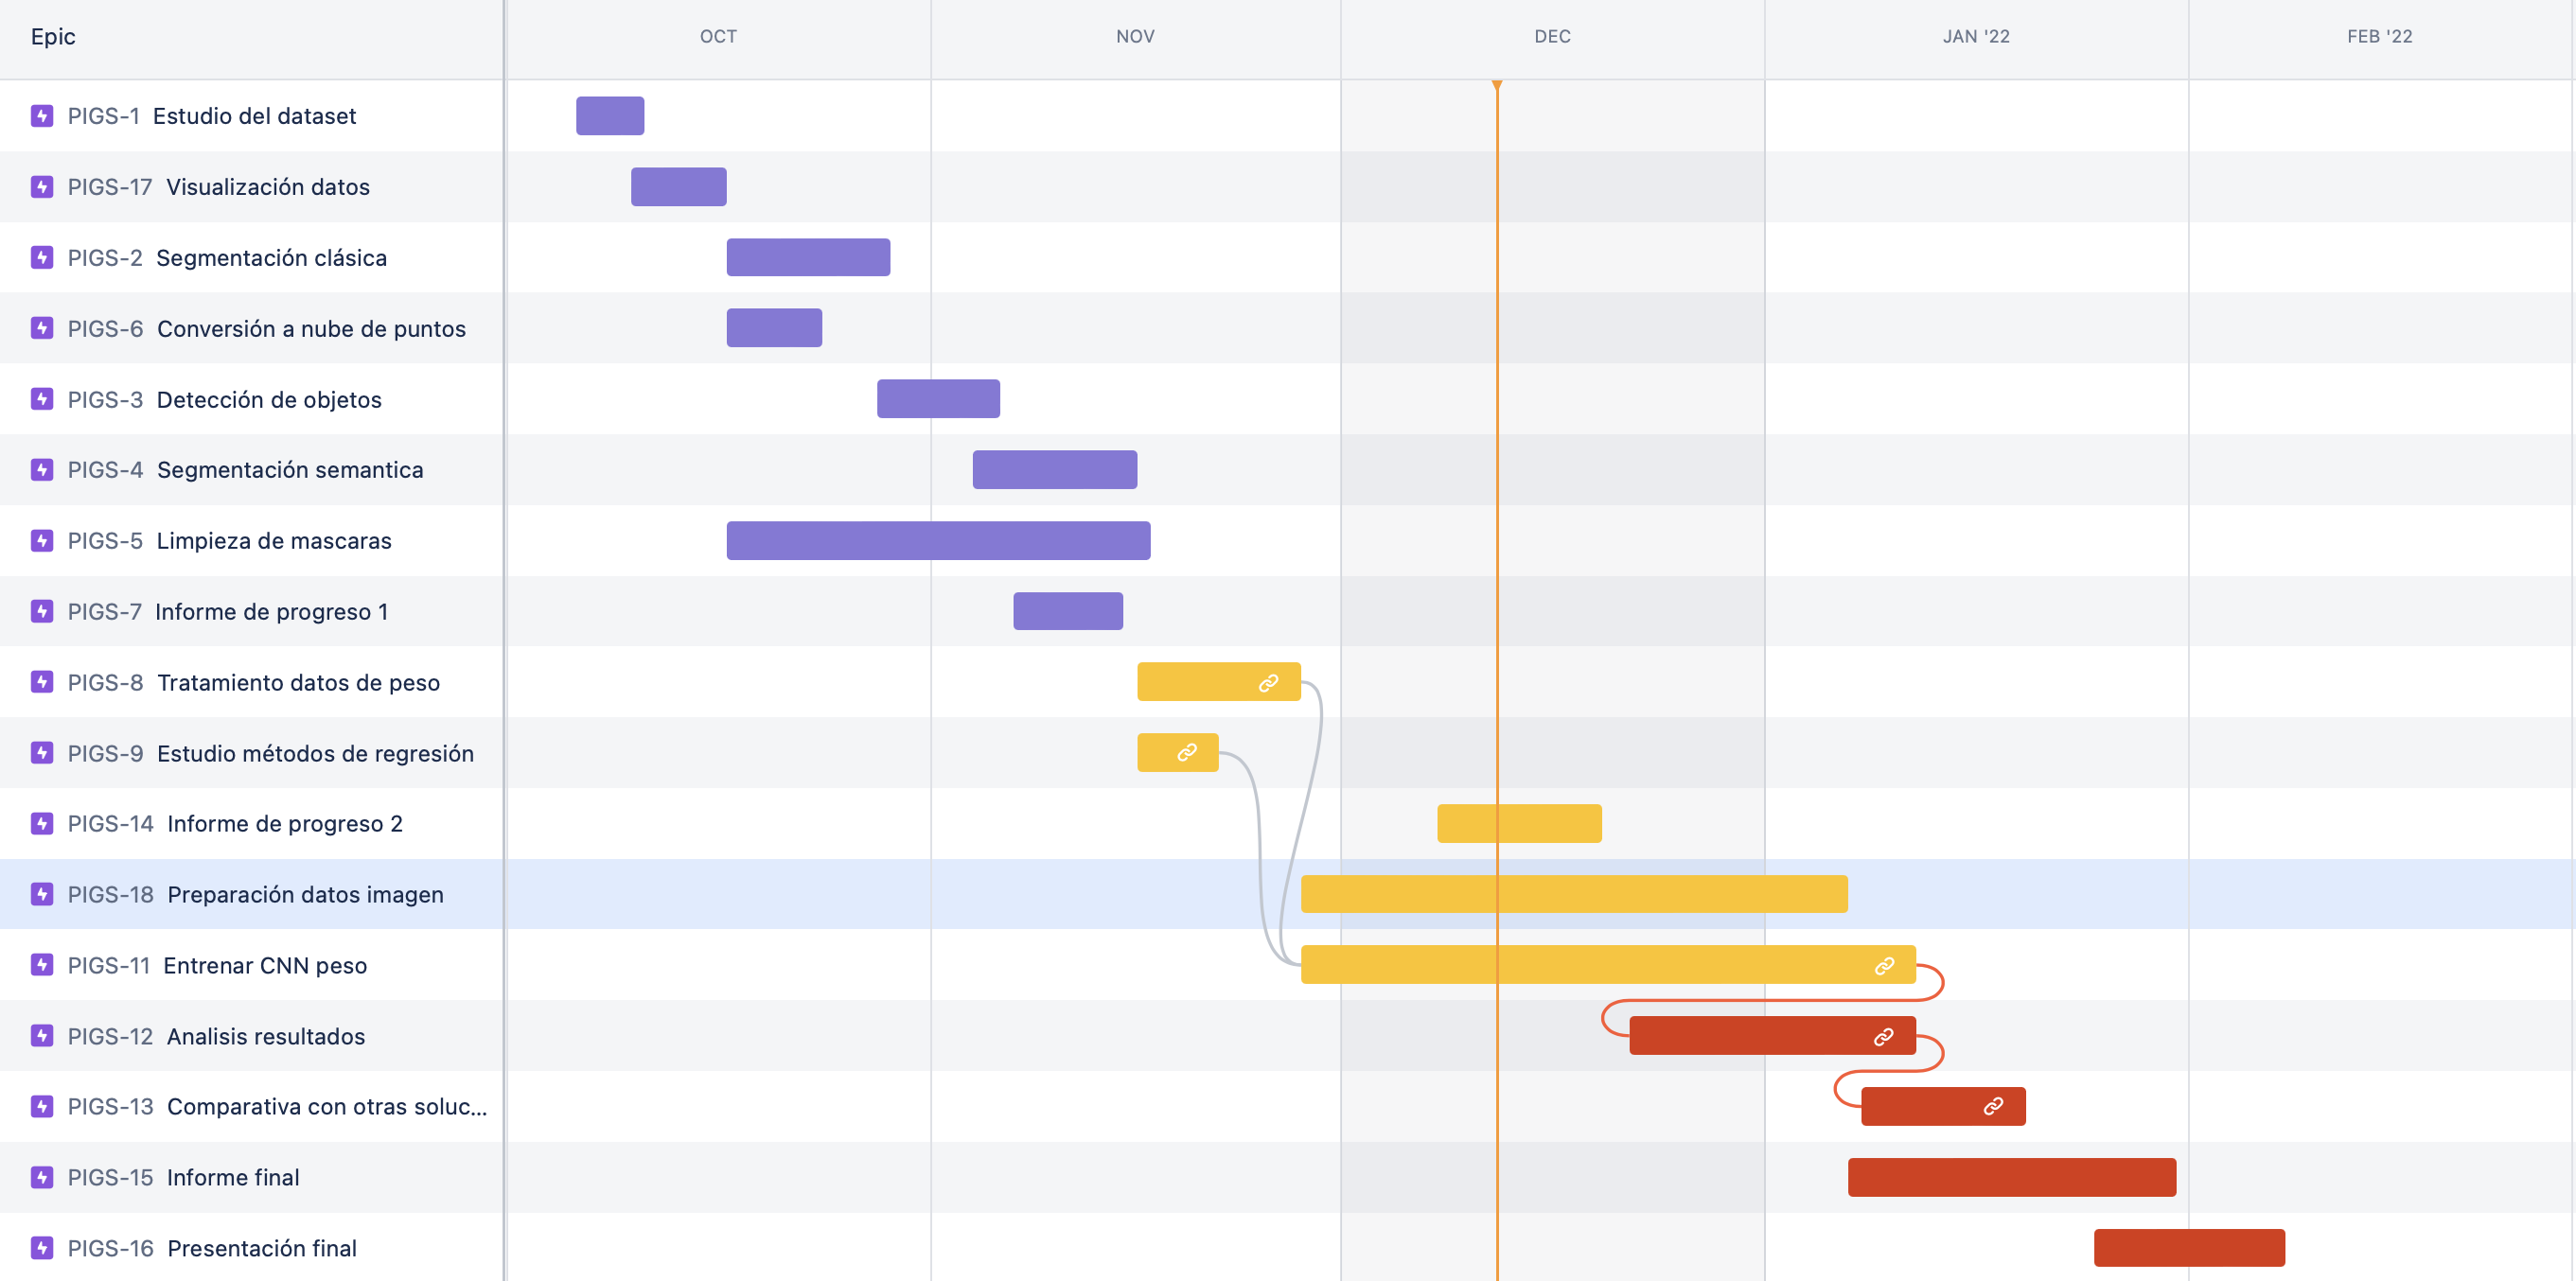
\includegraphics[width=1\textwidth]{05-TFG-template-latex/img/gantt.png}
\caption{Diagrama de Gantt planificación de tareas}
\label{g}

\end{figure}

\subsection{Predicción de los pesos}
\label{a3}


\begin{figure}[!htb]
\centering
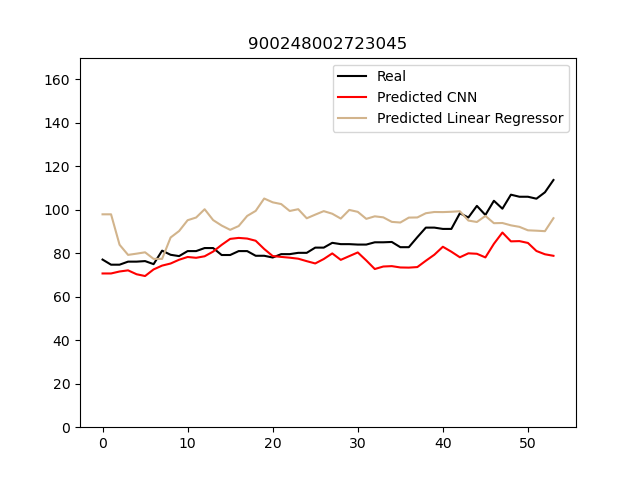
\includegraphics[width=0.9\textwidth]{05-TFG-template-latex/img/1.png}
\caption{Evolución del peso del cerdo 900248002723045}
\label{g}
\end{figure}

\begin{figure}[!htb]
\centering
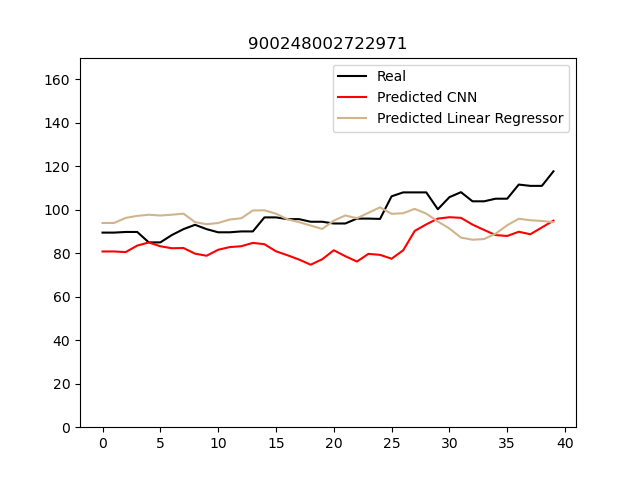
\includegraphics[width=0.9\textwidth]{05-TFG-template-latex/img/2.png}
\caption{Evolución del peso del cerdo 900248002722971}
\label{g}
\end{figure}

\begin{figure}[!htb]
\centering
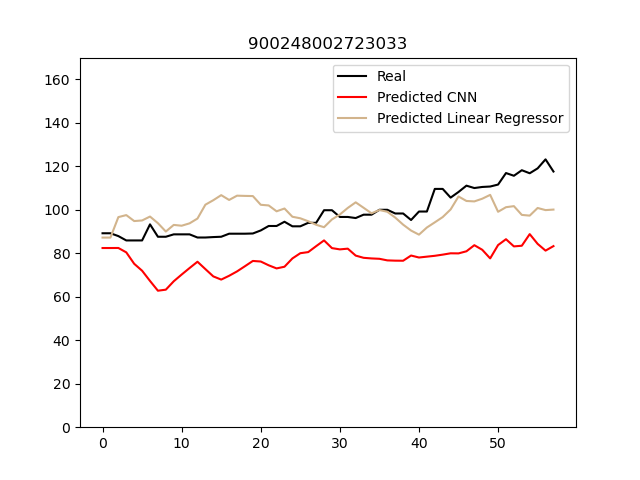
\includegraphics[width=0.9\textwidth]{05-TFG-template-latex/img/3.png}
\caption{Evolución del peso del cerdo 900248002723033}
\label{g}
\end{figure}

\end{document}

